In the figure below, what does \textit{x} equal in degrees?

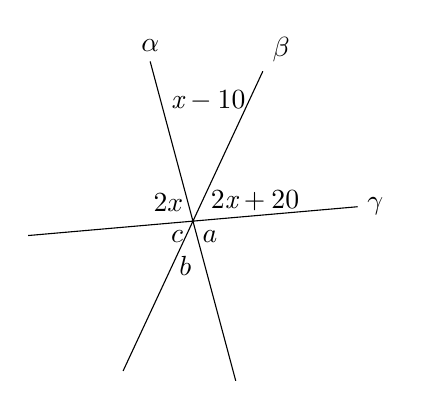
\begin{tikzpicture}[scale=1.05,rotate=5] 
\draw(240:2)--(60:2)node[anchor=south west]{$\beta$}; 
\draw(-80:2)--(100:2)node[anchor=south]{$\alpha$}; 
Looking at the figure below, what is the measure of \textit{x}?

\draw(-2,0)--(2,0)node[anchor=west]{$\gamma$}; 
\draw(0,0)node[anchor=south east]{$2x\degree$} 
node[anchor=north west]{$a\degree$} 
node[anchor=north east]{$c\degree$}; 
\draw(.1,0)node[anchor=south west]{$2\textit{x}+20\degree$}; 
\draw(0.29,1.2)node[anchor=south]{$\textit{x}-10\degree$}; 
\draw(-0.12,-.3)node[anchor=north]{$b\degree$}; 
\end{tikzpicture} 

\ifsat
	\begin{enumerate}[label=\Alph*)]
		\item   $20\degree$
		\item  $22\degree$ 
		\item  $34\degree$ %
		\item  $36\degree$ 
	\end{enumerate}
\else
\fi

\ifacteven
	\begin{enumerate}[label=\textbf{\Alph*.},itemsep=\fill,align=left]
		\setcounter{enumii}{5}
		\item   $20\degree$
		\item  $22\degree$ 
		\item  $34\degree$ %
		\addtocounter{enumii}{1}
		\item  $36\degree$ 
		\item  $44\degree$ 
	\end{enumerate}
\else
\fi

\ifactodd
	\begin{enumerate}[label=\textbf{\Alph*.},itemsep=\fill,align=left]
		\item   $20\degree$
		\item  $22\degree$ 
		\item  $34\degree$ %
		\item  $36\degree$ 
		\item  $44\degree$ 
	\end{enumerate}
\else
\fi

\ifgridin
  $34\degree$ %
		
\else
\fi

